\documentclass{article}
\usepackage{polski}
\usepackage[utf8]{inputenc}
\usepackage{float}

\title{Interpolacja Lagrange’a funkcji niesymetrycznej z
optymalizacją położeń węzłów.
}
\author{Wiktoria Zaczyk}
\date{22.04.2021}

\usepackage{natbib}
\usepackage{graphicx}
\graphicspath{ {./images/} }

\begin{document}

\maketitle

\section{Wstęp teoretyczny}

\newline\newline
\textbf{Interpolacja Lagrange’a}:
\newline
Iteracyjna metoda interpolacyjna; wyznaczamy przybliżone wartości interesującej nas funkcji iteracyjnie  z pomocą wcześniej wybranych
położeń węzłów. Dla każdego podanego punktu tworzymy wielomian węzłowy Lagrange’a :

\begin{center}
$\Phi_j(x) = \frac{(x-x_0)(x-x_1)\cdots (x-x_j_-_1)(x-x_j_+_1) \cdots (x-x_n) }{(x_j-x_0)(x_j-x_1)\cdots (x_j-x_j_-_1)(x_j-x_j_+_1) \cdots (x_j-x_n)}$
\end{center}
\newline
Wzór interpolacyjny Lagrange'a ma postać:

\begin{center}
    \[ W_n(x)=\sum_{i=0}^{n}y_i  \frac{ \prod_{j=0, j \neq i}^{n} (x-x_j) }{\prod_{j=0, j \neq i}^{n} (x_i-x_j)}\]
\end{center}
\newline
gdzie: $x_i$ to węzły interpolacji, $y_i = y(x_i)$ to wartości funkcji interpolowanej w węzłach, a
węzły indeksowane są i = 0, 1, . . . , n.\newline
\newline
\textbf{Efekt Rungego}:
\newline
Mówimy o nim gdy zadanie jest źle uwarunkowane, czyli kiedy zaczynają występować niedopasowania wielomianu interpolacyjnego na krańcach przedziału w wyniku zwiększnia liczby wezłów. Wynika to z oscylacji wielomianów wyższych rzędów. W celu zapobiegnięcia tego efektu stossuje się metody optymalizujące położenia węzłów.\newline
\newline
\textbf{Wielomiany Czebyszewa}:
\newline
układ wielomianów ortogonalnych tworzący bazę przestrzeni
wielomianów. Ich zera stanowią optymalne położenia węzłów w metodach interpolacyjnych
i można je wyznaczyć ze wzoru:

\begin{center}
    $x_m =\frac{1}{2} [(x_m_a_x-x_m_i_n)\cdot cos(\pi \frac{2i+1}{2n=1})+(x_m_a_x+x_m_i_n)]$
\end{center}

\section{Cel zadania}
Za zadanie mieliśmy wykonać interpolację funkcji $y(x)=\frac{x}{1+x^2}$ w przedziale $x\in [-3,8]$ dla stopni wielomianu n = 5, 10, 15 węzłów równomiernie i nierównomiernie rozłożonych korzystając z własności wielomianów Czebyszewa.

\section{Wyniki}
Metoda wyznaczająca
przybliżoną wartość funkcji w położeniu międzywęzłowym wykorzystując wielomian
interpolacyjny Lagrange’a.

\begin{figure}[h!]
\centering
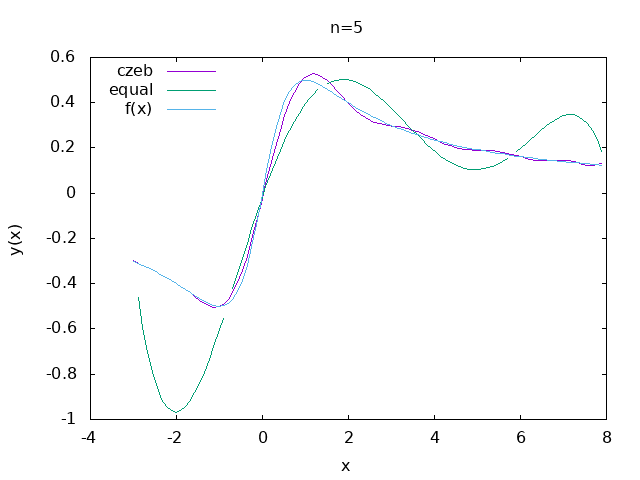
\includegraphics[width=8cm]{5.png}
\caption{Wykres funkcji interpolowanej i interpolującej dla n=5,  equal-przy klasycznym doborze położeń węzłów, czeb - przy zoptymalizowanym doborze położeń
węzłów}
\label{fig:obrazek 5}
\end{figure}

\begin{figure}[h!]
\centering
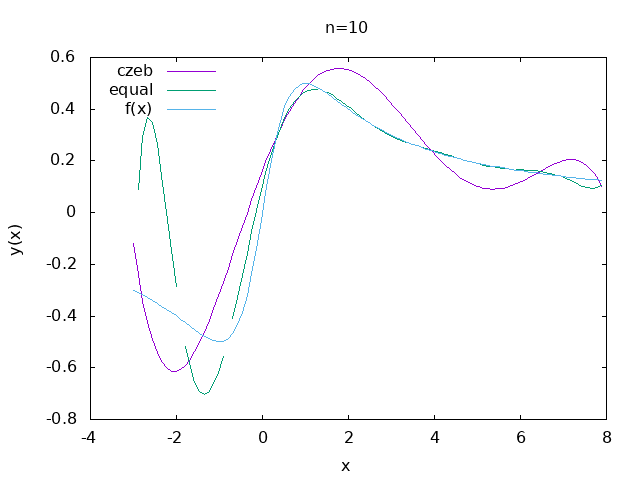
\includegraphics[width=8cm]{10.png}
\caption{Wykres funkcji interpolowanej i interpolującej dla n=10,  equal-przy klasycznym doborze położeń węzłów, czeb - przy zoptymalizowanym doborze położeń
węzłów}
\label{fig:obrazek 10}
\end{figure}

\begin{figure}[h!]
\centering
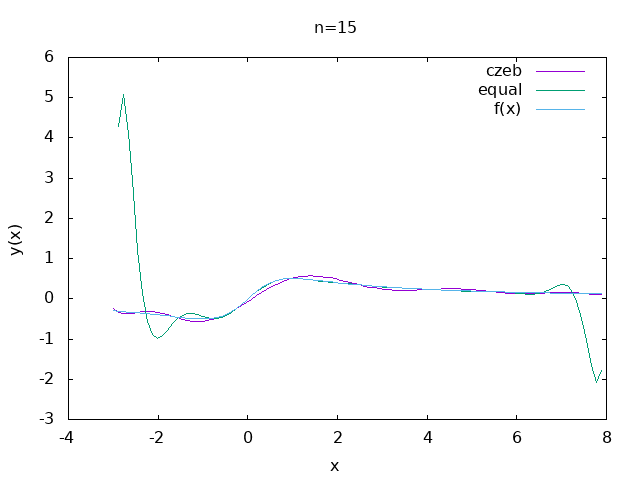
\includegraphics[width=8cm]{15.png}
\caption{Wykres funkcji interpolowanej i interpolującej dla n=15,  equal-przy klasycznym doborze położeń węzłów, czeb - przy zoptymalizowanym doborze położeń
węzłów}
\label{fig:obrazek 15}
\end{figure}

\newpage
\section{Wnioski}
\begin{flushleft}
Jak można zauważyć, zwiększenie liczby węzłów przy ich klasycznym doborze pozwoliło nam na zwiększenie dopasowania funkcji interpolującej w środku przedziału, jednak dla jego krańców można zauważyć silne oscylacje i niedokładności (efekt Rungego) Wyznaczając położenia węzłów jako zera wielomianów Czebyszewa, udało się uniknąć oscylacji na krańcach przedziału, jednak dla n=10 uzyskaliśmy gorsze przybliżenie . Przy braku stosowania wyrafinowanych metod optymalizacji pozycji węzłów występują charakterystyczne ”skoki” na krańcach przedziałów, interpolacja z tego powodu dość bardzo odbiega na tej części wykresu. Z pomocą przychodzi nam metoda Chebyshev’a, która skutecznie ogranicza odbicia i pozwala nam osiągnąć niemal idealną interpolację. Optymalizacja położeń węzłów daje nam znacznie lepsze wyniki na całym przedziale przybliżenia, za wyjątkiem jego środka.

\end{flushleft}

\end{document}

